\documentclass{scrartcl}

\usepackage{fontspec}
\usepackage[english]{babel}
\usepackage{lipsum}
\usepackage[paperheight=16in,paperwidth=9in,landscape]{geometry}
\usepackage[linktoc=all]{hyperref}
\usepackage{graphicx}
\hypersetup{
    colorlinks,
    citecolor=black,
    filecolor=black,
    linkcolor=black,
    urlcolor=black
}

\setmainfont[
  BoldFont={SFNSText-Bold.otf}, 
  ItalicFont={SFNSText-RegularItalic.otf},
  BoldItalicFont={SFNSText-BoldItalic.otf}
]{SFNSText-Regular.otf}

\newfontfamily\ClashGroteskBold{ClashGrotesk-Bold.ttf}
\newfontfamily\ClashGroteskSemibold{ClashGrotesk-Semibold.ttf}

\setkomafont{title}{\ClashGroteskSemibold}
\addtokomafont{section}{\ClashGroteskSemibold\Huge}

\setkomafont{sectionentry}{\sffamily\large}
\setkomafont{partentry}{\sffamily\normalsize}

\newcommand{\HUGE}{\fontsize{72}}
\newcommand{\pagetitle}[1]{{\ClashGroteskSemibold\Huge #1} \\}
\newcommand{\sectionpage}[1]{
  \pagebreak
  \vspace{7.5in}
  \vspace*{\fill}

  #1

  \vspace*{\fill}
}

\newcommand{\normalpage}[1]{
  \pagebreak
  #1}

\setlength{\parindent}{0pt}

\title{}
\author{Attila Pinter}
\date{}

\begin{document}
\large

\begin{titlepage}

	\vspace{7.5in}
	\vspace*{\fill}
	\begin{center}

		{\Huge \ClashGroteskSemibold Making a playable simulation of markets and organisations}\\

		\bigskip

		\parbox{0.8235\textwidth}{
			Kantonsschule im Lee Winterthur \\
			Maturitätsarbeit HS 2025/26 \\

			Attila Pinter, 4a \\
			Patrik Hknilcka \\

			\today
		}


	\end{center}

	\vspace*{\fill}
\end{titlepage}

\sectionpage{
	\section{Concept}
}

\sectionpage{
	\begin{center}
		
\includegraphics[width=0.5\textwidth]{Google-Logo-3014348739.png}
	\end{center}
}

\sectionpage{
	\begin{center}
		
\includegraphics[width=0.5\textwidth]{EA_logo_Signature-1645937650.jpg}
	\end{center}
}

\sectionpage{
	\begin{center}
		
\includegraphics[width=0.5\textwidth]{Nestle-Emblema-3312328101.png}
	\end{center}
}

\sectionpage{
	{\Huge Kennt ihr diese Firmen?}
}
\sectionpage{
	{\Huge Mögt ihr die?}
}

\sectionpage{
	{\Huge Wollt ihr CEO von diesen Firmen sein?}
}

\sectionpage{
	{\Huge Ja?}
		{\Huge Nein?}
		{\Huge Nein?}
}

\sectionpage{
	{\Huge Doch!}

	Ihr müsst :)
}

\normalpage{
	\pagetitle{Concept}

	\vspace*{\fill}
	\parbox{\textwidth}{
		{\LARGE Ein videospiel erstellen, wo Spieler Firmen gründen, Prudukte herstellen und gegeneinander konkurrieren.}
	}

	\vspace*{\fill}
}

\normalpage{
	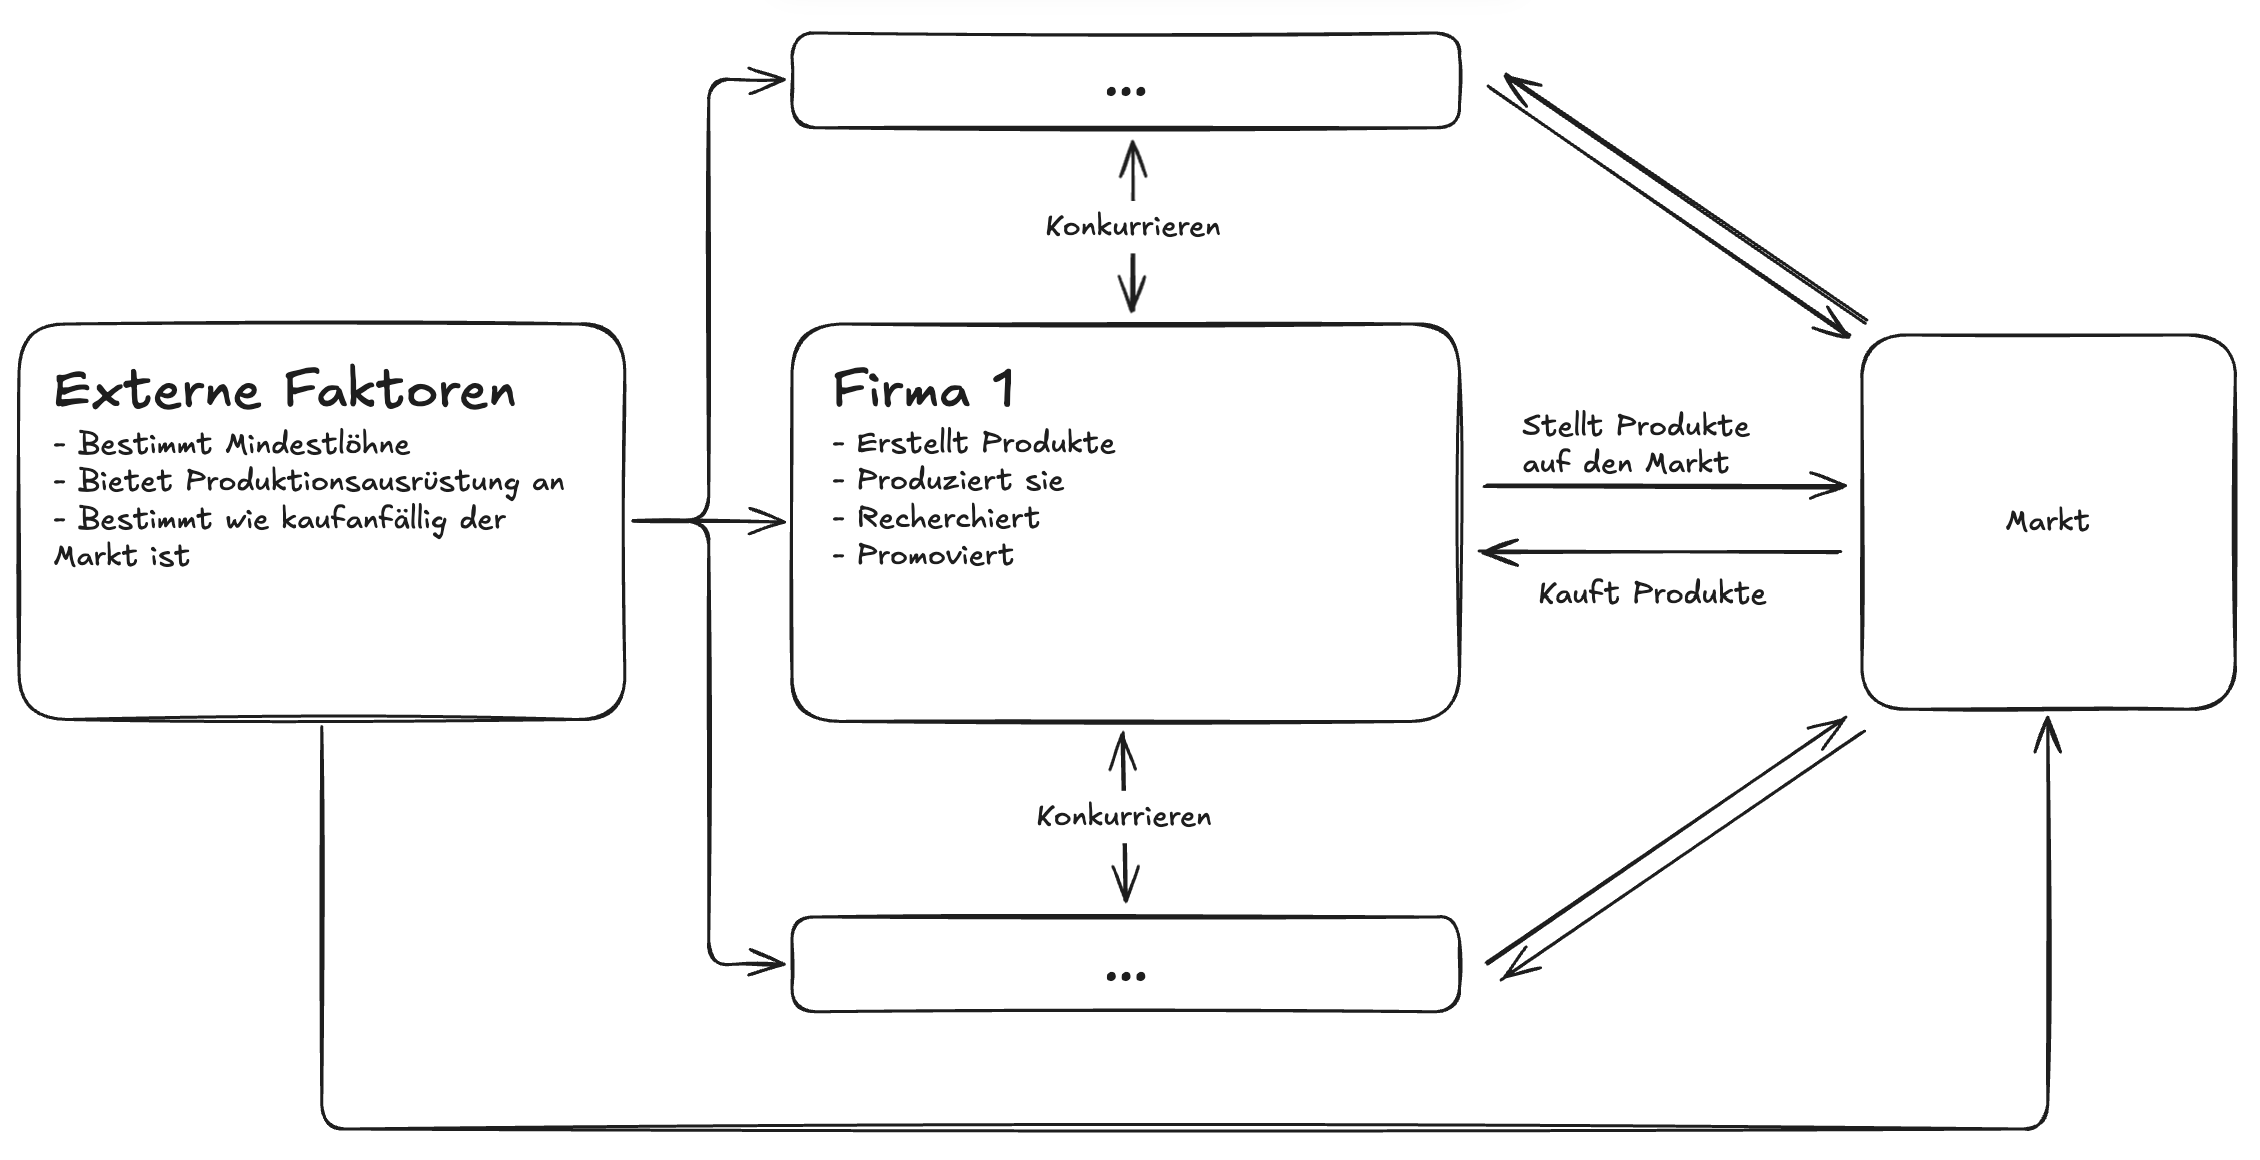
\includegraphics[width=\textwidth]{conceptualStructure.png}
}

\normalpage{
	\pagetitle{Ziel des Spiels: }

	\vspace{5cm}
	\parbox{\textwidth}{
		{\Huge \textbf{Die letze Firma auf den Markt zu sein.}

				Man kann auf 2 verscchiedene Wege verlieren:
				\begin{enumerate}
					\item{Man kann bankrupt gehen.}
					\item{Eine andere Firma kauft einen kontrollierenden Anteil der Firma.}
				\end{enumerate}

				\vspace*{\fill}
			}
	}
	\vspace*{\fill}
}

\end{document}
